\subsection{Kriging-based Surrogate for Parameter Calibration}

%%%%%%%%%%%%%%%%%%%%%%%%%%%%%%%%%%%%%%%%%%%%%%%%%%%%%%%%%%%%%%%%%%%%%%%%%%%%%%%%%%%%%%%%
\begin{frame}
\frametitle{FGR Parameters Used for Calibration}

\begin{itemize}
  \item Through a thorough literature review and discussions with Pastore et. al. the following parameters and uncertainty ranges are considered for calibration.
\end{itemize}

\begin{table} 
\tiny
\centering
\begin{tabular}{||c|c|c|c|c||} 
\hline \hline
\textbf{Description} & \textbf{Symbol} & \textbf{Lower Bound} & \textbf{Upper Bound} & \textbf{Scaled} \\ \hline
Initial Fuel Grain Radius & $r_{g,0}$  $\left[ m\right]$  & 2.0E-6 & 15.0E-6 & no \\ \hline
Fuel Porosity               & $P_f$      & 0.0      & 0.1      & no \\ \hline
Surface Tension           & $\gamma$  $\left[ J\cdot m^{-2}\right]$ & 0.5     & 1.0      & no \\ \hline
Temperature               & $T$          & 0.95   & 1.05     & yes \\ \hline
Fuel Grain Radius         & $r_g$       & 0.4     & 1.6      & yes \\ \hline
Vacancy Diffusion Coef.  & $D_v$ $\left[ m^{2}\cdot s^{-1}\right]$      & 0.1      & 10.0     & no \\ \hline
Resolution Parameter    & $b$ $\left[ s^{-1}\right]$        & 0.1      & 10.0     & no \\ \hline
Intra-granular Diffusion Coef. & $D_s$  $\left[ m^{2}\cdot s^{-1}\right]$ & 0.316 & 3.162   & no \\ 
\hline \hline
\end{tabular}
\end{table}

\end{frame}
%%%%%%%%%%%%%%%%%%%%%%%%%%%%%%%%%%%%%%%%%%%%%%%%%%%%%%%%%%%%%%%%%%%%%%%%%%%%%%%%%%%%%%%%
\begin{frame}
\frametitle{Sampling FGR Parameters}

\begin{itemize}
  \item The FGR parameters are randomly sampled 100 times and propagated through Bison.
\end{itemize}

\begin{figure}
  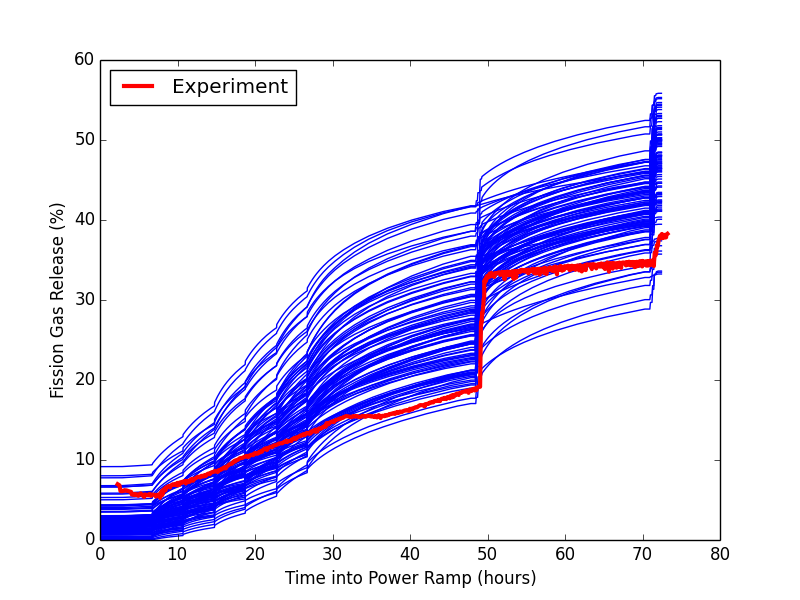
\includegraphics[width=0.75\textwidth]{/Users/yankovai/Documents/Thesis/Chapter4/fgr_simulations.png}
\end{figure}

\end{frame}
%%%%%%%%%%%%%%%%%%%%%%%%%%%%%%%%%%%%%%%%%%%%%%%%%%%%%%%%%%%%%%%%%%%%%%%%%%%%%%%%%%%%%%%%
\begin{frame}
\frametitle{Modeling Problem}

\begin{itemize}
  \item Each FGR simulation in Bison takes approximately an hour using 16 processors.
  \item We need a fast mapping from the FGR parameters to FGR kinetics time series output by Bison for calibration.
  \item Surrogate methods described previously are really designed for acting on scalar quantities. We have a time series.
  \item Build a surrogate at each time-step? Inefficient. Unstable.  
  \item Apply Principal Component Analysis (PCA) to model variations in FGR kinetics. 
\end{itemize}

\end{frame}
%%%%%%%%%%%%%%%%%%%%%%%%%%%%%%%%%%%%%%%%%%%%%%%%%%%%%%%%%%%%%%%%%%%%%%%%%%%%%%%%%%%%%%%%
\begin{frame}
\frametitle{Applying PCA}

\begin{columns}
 \begin{column}{0.5\textwidth}
  \centering
  Eigenvalues
  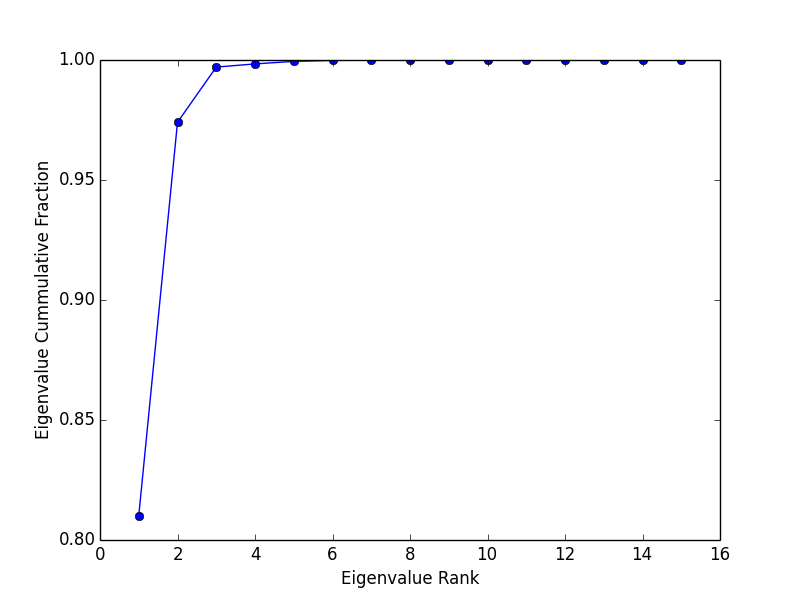
\includegraphics[width=1.\textwidth]{/Users/yankovai/Documents/Thesis/Chapter4/fgr_evals.png}
 \end{column}
 \begin{column}{0.5\textwidth}
  \centering
  Top three eigenvectors
  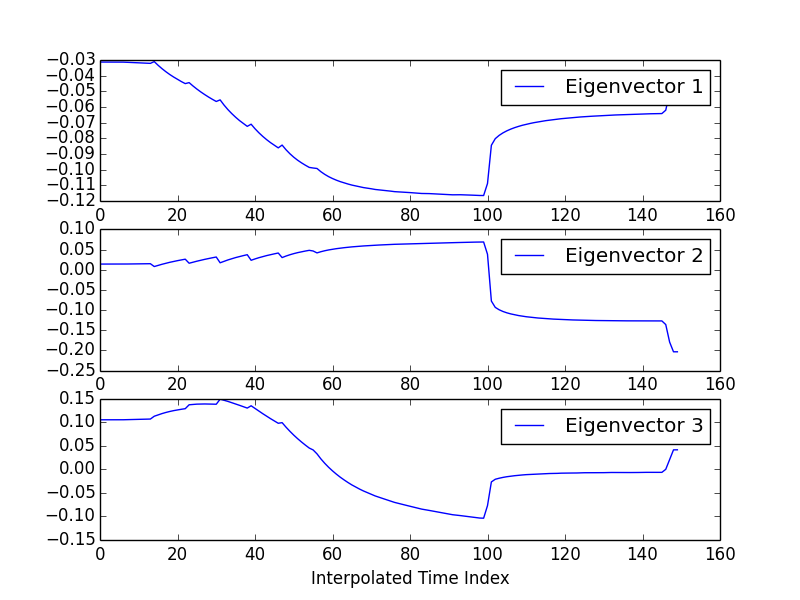
\includegraphics[width=1.\textwidth]{/Users/yankovai/Documents/Thesis/Chapter4/fgr_evecs.png}
 \end{column}
\end{columns}

\end{frame}
%%%%%%%%%%%%%%%%%%%%%%%%%%%%%%%%%%%%%%%%%%%%%%%%%%%%%%%%%%%%%%%%%%%%%%%%%%%%%%%%%%%%%%%%
\begin{frame}
\frametitle{Insights with PCA}

\begin{itemize}
  \item The top three principal components account for over 99\% of the variance in the simulated FGR kinetics.
  \item Correlate the variation in FGR parameter values with each of the principal components to see which parameters are the drivers of the variance.
\end{itemize}

\begin{figure}
  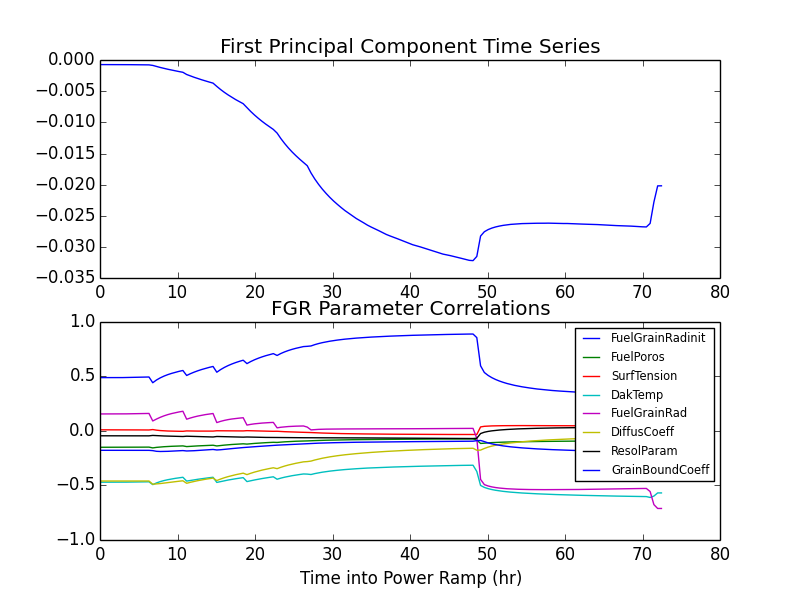
\includegraphics[width=0.6\textwidth]{/Users/yankovai/Documents/Thesis/Chapter4/firstPrincComp_FGR_Correlations.png}
\end{figure}

\end{frame}
%%%%%%%%%%%%%%%%%%%%%%%%%%%%%%%%%%%%%%%%%%%%%%%%%%%%%%%%%%%%%%%%%%%%%%%%%%%%%%%%%%%%%%%%
\begin{frame}
\frametitle{Using PCA for Surrogate Construction}

\begin{itemize}
  \item Through PCA we showed you can effectively represent any Bison FGR kinetics time series using three principal components.
  \item Use Kriging to construct three surrogates, each of which maps the FGR parameters $R^i$ to one of the 3 PCA expansion coefficients $\hat{p}_{ij}$ corresponding to the principal components $X_j$ for $j\in\left(1,2,3\right)$.
\end{itemize}

\begin{equation}
 \hat{\mathcal{F}}^{i}(R^i) = \hat{p}_{i1}\left(R^i\right) X_1 + \hat{p}_{i2}\left(R^i\right) X_2 + \hat{p}_{i3}\left(R^i\right) X_3 + \mu \nonumber  
\end{equation}

\begin{equation}
 \sigma_{ \hat{\mathcal{F}}^i }^2 = \sigma_{\hat{p}_{i1}}^2 X_1^2 + \sigma_{\hat{p}_{i2}}^2 X_2^2 + \sigma_{\hat{p}_{i3}}^2 X_3^2  \nonumber
\end{equation}

\end{frame}
%%%%%%%%%%%%%%%%%%%%%%%%%%%%%%%%%%%%%%%%%%%%%%%%%%%%%%%%%%%%%%%%%%%%%%%%%%%%%%%%%%%%%%%%
\begin{frame}
\frametitle{Cross Validation}

\begin{itemize}
  \item 100 independent Bison simulations of the Ris\o~ AN3 power ramp are obtained (test set).
  \item PCA expansion coefficient surrogates are built on original 100 simulations (train set). 
  \item Both inverse and logarithmic transforms are applied without increase in prediction accuracy.
\end{itemize}

\begin{figure}
  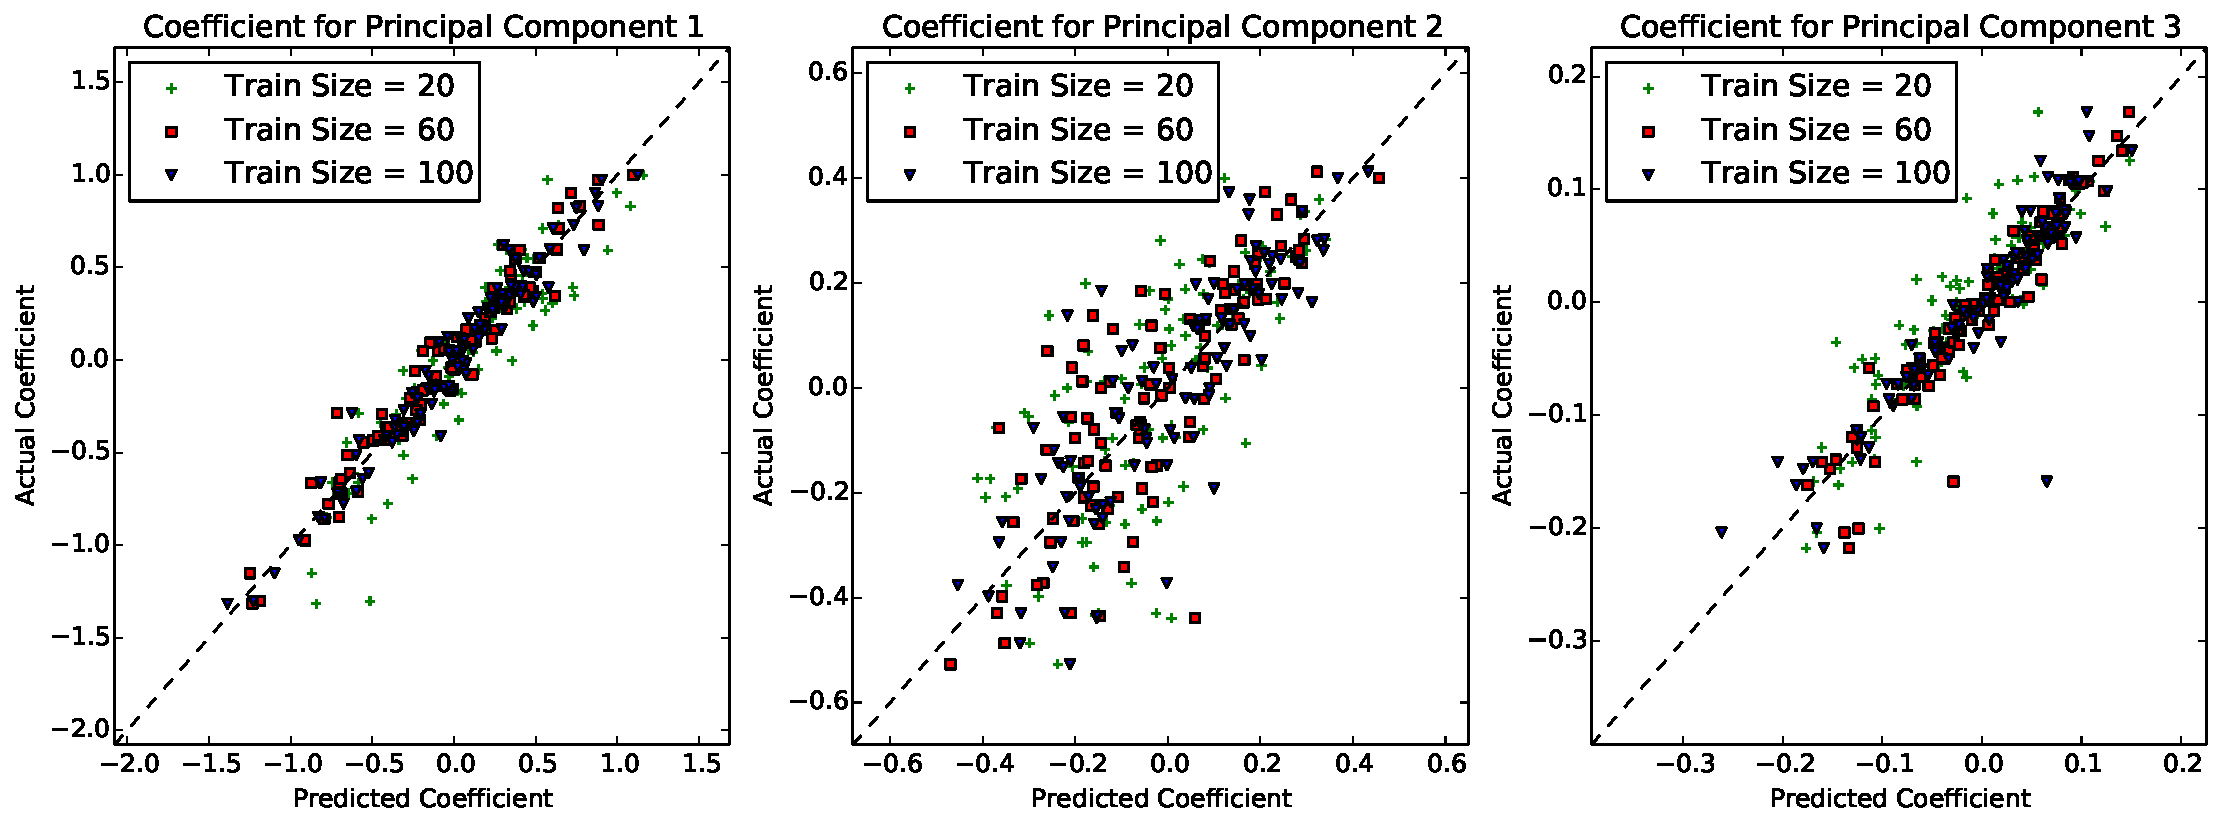
\includegraphics[width=0.9\textwidth]{/Users/yankovai/Documents/Thesis/Chapter4/xval_45degree.pdf}
\end{figure}

\end{frame}
%%%%%%%%%%%%%%%%%%%%%%%%%%%%%%%%%%%%%%%%%%%%%%%%%%%%%%%%%%%%%%%%%%%%%%%%%%%%%%%%%%%%%%%%
\begin{frame}
\frametitle{Cross Validation}

\begin{itemize}
  \item Standardized cross-validated residual plotted.

\begin{equation}
 \frac{ p_{ij} - \hat{p}_{ij} }{ \sigma_{\hat{p}_{ij}} } \nonumber
\end{equation}  

\end{itemize}

\begin{figure}
  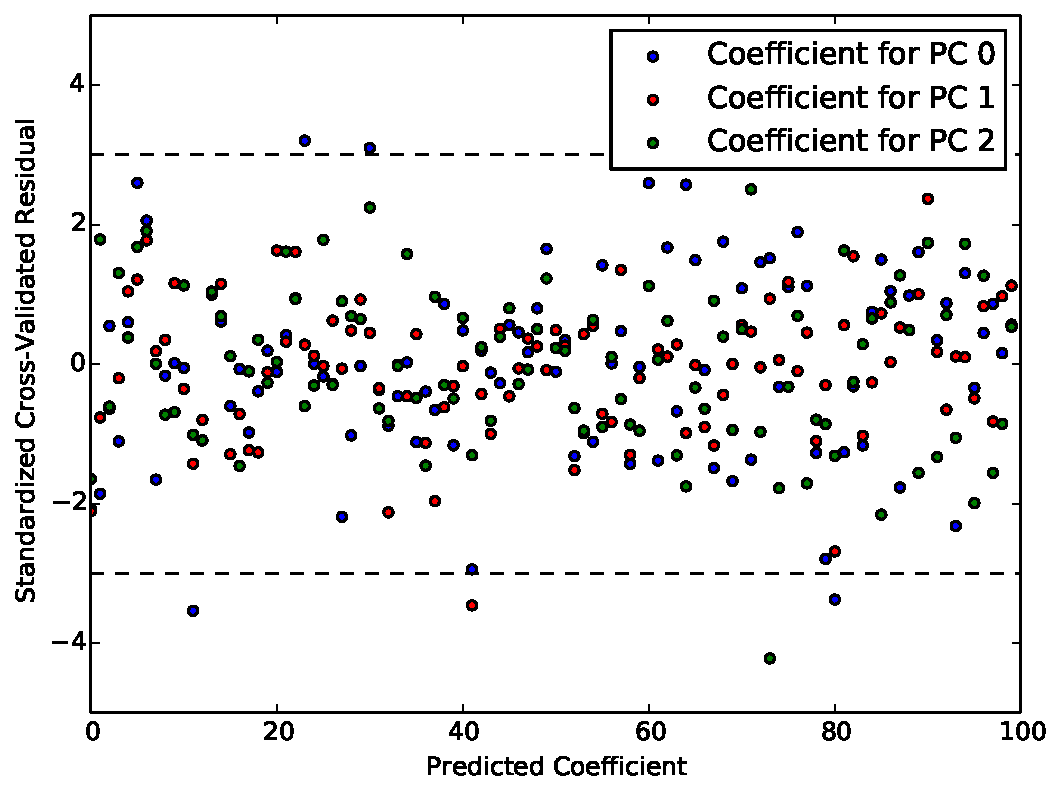
\includegraphics[width=0.6\textwidth]{/Users/yankovai/Documents/Thesis/Chapter4/xval_3sig_band.pdf}
\end{figure}

\end{frame}
%%%%%%%%%%%%%%%%%%%%%%%%%%%%%%%%%%%%%%%%%%%%%%%%%%%%%%%%%%%%%%%%%%%%%%%%%%%%%%%%%%%%%%%%
\begin{frame}
\frametitle{Calibration of FGR Parameters}

\begin{itemize}
  \item To determine the error between predicted time series the RMSE is used as a cost function. 
  \item The objective of calibration is to find a set of fission gas release parameters such that the RMSE between prediction and experiment is minimized.
  \item Many potential algorithms to use for calibration (EGO, Nelder-Mead, COBYLA, Simplex, Newton-CG).
  \item To decide whether to use a global optimizer or local optimizer it's worthwhile to do some sensitivity analysis.  
\end{itemize}

\end{frame}
%%%%%%%%%%%%%%%%%%%%%%%%%%%%%%%%%%%%%%%%%%%%%%%%%%%%%%%%%%%%%%%%%%%%%%%%%%%%%%%%%%%%%%%%
\begin{frame}
\frametitle{Sensitivity Analysis Using FGR Kinetics Surrogate}

\begin{itemize}
  \item Morris' Algorithm is initially applied to get a sense of which parameters interact with others and which have the largest main effects.
  \item A total of 4500 evaluations of the FGR kinetics surrogate are required to produce the plot below:
\end{itemize}

\begin{figure}
  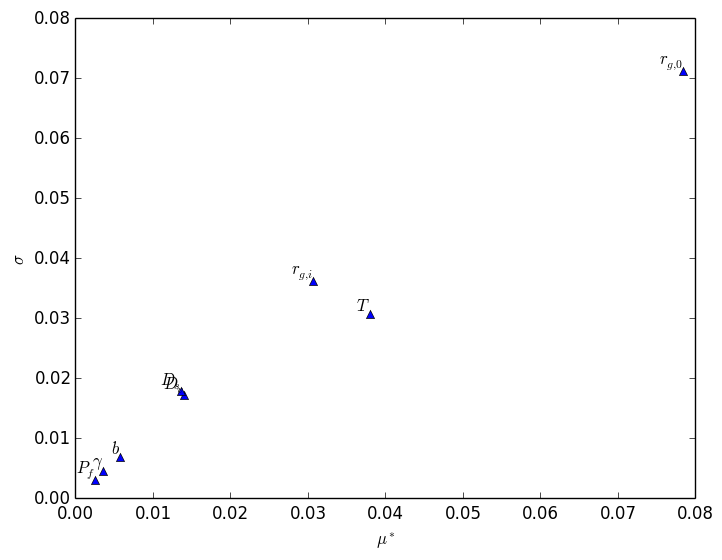
\includegraphics[width=0.6\textwidth]{/Users/yankovai/Documents/Thesis/Chapter4/fgr_morris.png}
\end{figure}

\end{frame}
%%%%%%%%%%%%%%%%%%%%%%%%%%%%%%%%%%%%%%%%%%%%%%%%%%%%%%%%%%%%%%%%%%%%%%%%%%%%%%%%%%%%%%%%
\begin{frame}
\frametitle{Sensitivity Analysis Using FGR Kinetics Surrogate}

\begin{itemize}
  \item Main and total effect indices for the RMSE using the Sobol-Jansen algorithm. 
  \item A total of $10^5$ instances of the surrogate are used to estimate the indices.
\end{itemize}

\begin{figure}
  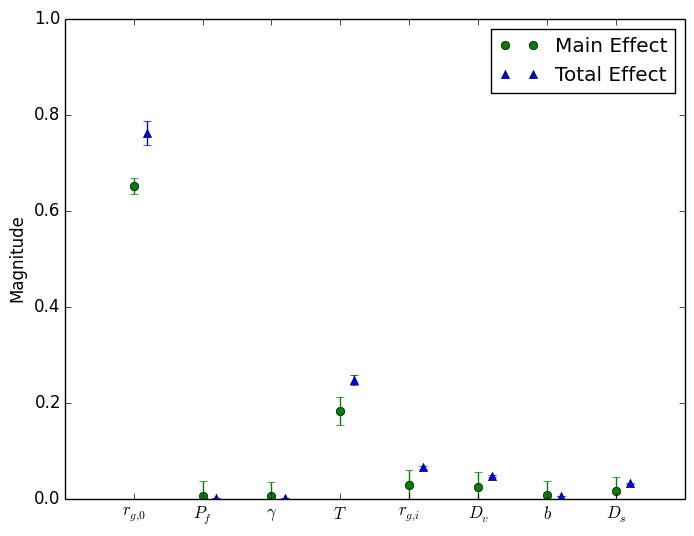
\includegraphics[width=0.6\textwidth]{/Users/yankovai/Documents/Thesis/Chapter4/sobol_indices.png}
\end{figure}

\end{frame}
%%%%%%%%%%%%%%%%%%%%%%%%%%%%%%%%%%%%%%%%%%%%%%%%%%%%%%%%%%%%%%%%%%%%%%%%%%%%%%%%%%%%%%%%
\begin{frame}
\frametitle{Sensitivity Analysis Using FGR Kinetics Surrogate}

\begin{itemize}
  \item Second order Sobol indices for the RMSE.
  \item A total of $3.7\times 10^5$ instances of the surrogate are used to estimate the indices.
\end{itemize}

\begin{figure}
  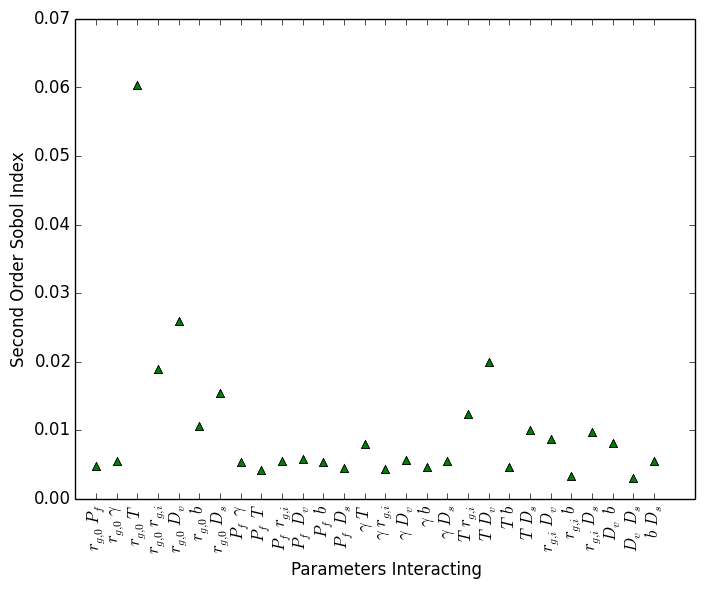
\includegraphics[width=0.6\textwidth]{/Users/yankovai/Documents/Thesis/Chapter4/sobol_2nd_order.png}
\end{figure}

\end{frame}
%%%%%%%%%%%%%%%%%%%%%%%%%%%%%%%%%%%%%%%%%%%%%%%%%%%%%%%%%%%%%%%%%%%%%%%%%%%%%%%%%%%%%%%%
\begin{frame}
\frametitle{Calibrating the FGR Parameters}

\begin{itemize}
  \item Given the presence of strong interaction among the fission gas release parameters it is unlikely a global RMSE minimum can be found in reasonable time. 
  \item A locally optimal solution can be found using the COBYLA algorithm. 
  \item The COBYLA algorithm is of the simplex variety that does not require any gradient information while allowing for constraints to be placed on both the search parameters and objective function. 
  \item For this problem it is necessary to not allow fission gas parameters that result in negative fission gas release values in predicted time series. 
\end{itemize}

\end{frame}
%%%%%%%%%%%%%%%%%%%%%%%%%%%%%%%%%%%%%%%%%%%%%%%%%%%%%%%%%%%%%%%%%%%%%%%%%%%%%%%%%%%%%%%%
\begin{frame}
\frametitle{Calibrating the FGR Parameters}

\begin{itemize}
  \item Optimization algorithms such as COBYLA are sensitive to initial search conditions.
  \item The algorithm is executed 100 different times, with each execution being seeded by one of the 100 LHS used to construct the expansion coefficient surrogates. 
  \item Such a procedure increases the probability of finding a true minimum RMSE and not one existing in a flat space. 
  \item The minimum RMSE found was 2.94\%.
  \item To identify the locally minimum RMSE some $10^5$ instances of the surrogate were required. 
\end{itemize}

\end{frame}
%%%%%%%%%%%%%%%%%%%%%%%%%%%%%%%%%%%%%%%%%%%%%%%%%%%%%%%%%%%%%%%%%%%%%%%%%%%%%%%%%%%%%%%%
\begin{frame}
\frametitle{Calibrating the FGR Parameters}

\begin{figure}
  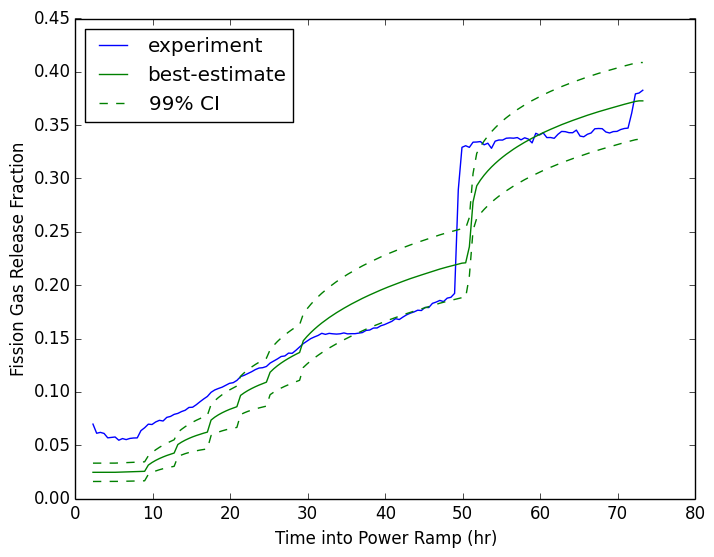
\includegraphics[width=0.75\textwidth]{/Users/yankovai/Documents/Thesis/Chapter4/fgr_best_estimate.png}
\end{figure}

\end{frame}
%%%%%%%%%%%%%%%%%%%%%%%%%%%%%%%%%%%%%%%%%%%%%%%%%%%%%%%%%%%%%%%%%%%%%%%%%%%%%%%%%%%%%%%%
\begin{frame}
\frametitle{Calibrating the FGR Parameters}

\begin{itemize}
  \item Optimal parameter values, with each parameter scaled to the unit hypercube, found for each of the 100 COBYLA seedings is summarized in a boxplot.
  \item The length of the whiskers implies strong non-linear interaction effects.
\end{itemize}

\begin{figure}
  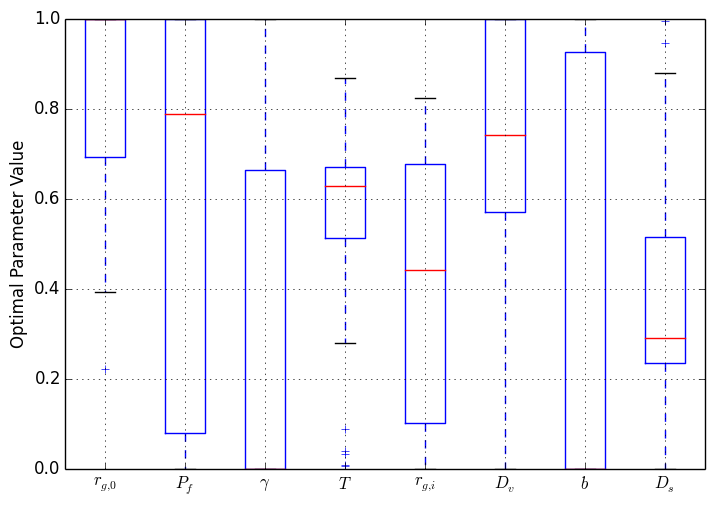
\includegraphics[width=0.6\textwidth]{/Users/yankovai/Documents/Thesis/Chapter4/optimal_params_boxplot.png}
\end{figure}

\end{frame}
%%%%%%%%%%%%%%%%%%%%%%%%%%%%%%%%%%%%%%%%%%%%%%%%%%%%%%%%%%%%%%%%%%%%%%%%%%%%%%%%%%%%%%%%
\begin{frame}
\frametitle{Smoothing Experimental Data}

\begin{itemize}
  \item At some points in the experimental data the total fission gas release decreases, which is not physical. 
  \item However, with only a single time series measurement there is no way of assigning uncertainties to fission gas release values measured at different times throughout the power ramp. 
  \item In an attempt to smooth the experimental data local polynomial regression was applied with the minimal amount of smoothing necessary to make the fission gas release time series strictly monotonically increasing. 
  \item The locally minimal RMSE was calculated to be 2.49\%, which is a 15.5\% reduction in RMSE from when raw experimental data is utilized.
\end{itemize}

\end{frame}
%%%%%%%%%%%%%%%%%%%%%%%%%%%%%%%%%%%%%%%%%%%%%%%%%%%%%%%%%%%%%%%%%%%%%%%%%%%%%%%%%%%%%%%%
\begin{frame}
\frametitle{Smoothing Experimental Data}

\begin{figure}
  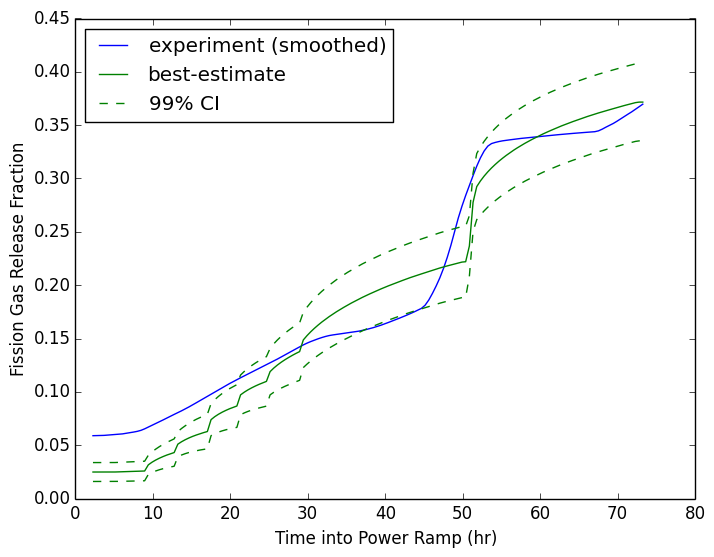
\includegraphics[width=0.75\textwidth]{/Users/yankovai/Documents/Thesis/Chapter4/best_estimate_smooth.png}
\end{figure}

\end{frame}
